%%
%% Commands for TeXCount
%TC:macro \cite [option:text,text]
%TC:macro \citep [option:text,text]
%TC:macro \citet [option:text,text]
%TC:envir table 0 1
%TC:envir table* 0 1
%TC:envir tabular [ignore] word
%TC:envir displaymath 0 word
%TC:envir math 0 word
%TC:envir comment 0 0
%%
%%
%% The first command in your LaTeX source must be the \documentclass command.
\documentclass[sigplan,screen]{acmart}
\setcopyright{none} 
\begin{document}

%%
%% The "title" command has an optional parameter,
%% allowing the author to define a "short title" to be used in page headers.
\title{Implementación de un método de recomendación de POI utilizando Bi-LSTM Attention}

%%
%% The "author" command and its associated commands are used to define
%% the authors and their affiliations.
%% Of note is the shared affiliation of the first two authors, and the
%% "authornote" and "authornotemark" commands
%% used to denote shared contribution to the research.
\author{Bianca Del Solar Medrano}
\email{bsdelsolar@uc.cl}
\affiliation{%
  \institution{Pontificia Universidad Catolica de Chile}
  \city{Santiago}
  \country{Chile}
}

\author{Rafael Fernandez}
\email{rafafdz@uc.cl}
\affiliation{%
  \institution{Pontificia Universidad Catolica de Chile}
  \city{Santiago}
  \country{Chile}
}

%%
%% The abstract is a short summary of the work to be presented in the
%% article.
\begin{abstract}
En este trabajo se implementó un método basado en el paper \cite{wang2021poi}. Este propone el uso de Bi-LSTM para recomendar la siguiente localidad de interés para un usuario, dado el historial de lugares visitados. Se entrenan embeddings para transformar las localidades en vectores. Luego cada secuencia de usuario se pasa a través, de una capa Bi-LSTM y una capa de Attention. Luego se concatena con información del usuario y sus amigos. Finalmente pasa por una capa fully connected, donde se obtienen  las latitudes y longitudes, además de los embeddings de locaciones. Estos son filtrados por una funcion de pérdida compuesta que permite acotar los resultados a localidades cercanas a la ubicación del usuario.
\end{abstract}

%%
%% Keywords. The author(s) should pick words that accurately describe
%% the work being presented. Separate the keywords with commas.
\keywords{Sistemas de Recomendación, Bi-LSTM, Embeddings, LBSN}

\maketitle

\section{Introducción}
Actualmente contamos con sistemas de geolocalización inmersos en nuestros dispositivos móviles, gracias a ello es posible incorporar acciones como compartir ubicaciones o marcar puntos de interés en los mapas, y/o redes sociales, esto es lo que conocemos como LBSN (location-based social networks) \cite{qian2018time}. En estos sistemas, los usuarios pueden iniciar sesión e indicar que se ha llegado a un punto de interés (POI). 
Sin embargo, cuando se habla de recomendar un POI, se considera algo más complejo que un sistema de recomendación clásico \cite{si2019adaptive}. En comparación con ver películas o comprar en línea, las personas que visitan un lugar en el mundo real requerirán más tiempo y esfuerzo, es por ello que este es uno de los problemas de los cuales existen pocos datos, ya que conceptualmente hablando los usuarios tienden a no compartir ubicaciones para no dejar registros personales y proteger su privacidad \cite{xiong2020go}. El segundo problema es \textbf{cold-start} que se encuentra comúnmente en las tareas del sistema recomendadas. Existen principalmente tres tipos de tareas de recomendación de puntos de interés: las ubicaciones que nunca se han visitado se denominan puntos de interés de arranque en frío. Los usuarios que nunca han visitado ninguna ubicación se denominan usuarios de \textbf{cold-start}. Los usuarios que se mudan de un lugar a otro desconocido para vivir o viajar también encontrarán problemas de \textbf{cold-start}\cite{qian2019spatiotemporal}. Finalmente, está el tema de las preferencias dinámicas del usuario. Es decir, las preferencias del usuario cambiarán con el paso del tiempo y los cambios en el entorno \cite{xing2018points}. Por lo tanto, es necesario considerar una variedad de factores que influyen para mejorar el desempeño de la recomendación de esta tarea.

Es por ello que basado en \cite{wang2021poi} se considerar los siguientes puntos importantes en base al método propuesto, considerando los siguientes problemas:
\begin{itemize}
\item \textbf{Dispersión de datos}: apuntando a este problema, el paper propone un modelo de embeddings que se utiliza para cuantificar la información inicial. Y para modelos de características de baja dimensión de diferentes fuentes de información, se utilizan diferentes capas de redes neuronales para extraer características de alta dimensión. Esto garantiza aún más la precisión de la siguiente recomendación de POI.\\

\item \textbf{Cambio de intereses de los usuarios } El paper propone el uso de un modelo que puede extraer las preferencias a largo plazo del usuario de todas las secuencias históricas de inicio de sesión de POI del usuario. Al mismo tiempo, se enfoca en las preferencias a corto plazo en la secuencia de inicio de sesión de PDI actual. Capte de manera integral los cambios dinámicos de las preferencias del usuario y mejore la eficiencia y precisión de las recomendaciones.
\end{itemize}

El trabajo se organiza de la siguiente manera. En la sección 2, se habla del estado del arte investigado, en la sección 3, se mencionará el detalles del dataset utilizado, en la sección 4, se detallará en profundidad la metodología utilizada, en la sección 5 se mostrarán los resultados obtenidos , y finalmente en la sección 6 se muestra la evaluación realizada del método propuesto y las conclusiones en la sección 7.

\section{Estado del Arte}
En la siguiente sección se muestran algunos avances encontrados en la recomendación de localizaciones de usuarios. 
\begin{itemize}
    \item \textbf{Baseline 1} Matriz de factorización x Matriz multi-etiqueta \cite{zhang2019fused}: La matriz de factorización es más eficiente al tratar de predecir valores faltantes de alguna tabla basado en la preferencia del usuario, mientras que la matriz multietiqueta, compara el usuario con una serie de etiquetas, el beneficio de esto es que es posible encontrar relaciones ocultas entre algún usuario y un punto de interés, por lo que en este paper se trata de hacer una combinación entre estos dos métodos para obtener un mejor resultado. Para hacer una evaluación del modelo se utilizaron métricas como RMSE y MAE donde se hizo 4 pruebas diferentes con distinta cantidad de sparsity para cada una de las métricas obteniendo un valor entre 0.862 a 0.928 para RMSE, y un valor entre 0.709 a 0.731 para MAE. \\

    \item \textbf{Baseline 2} DRLM\cite{huang2020deep}: Dos problemas conocidos de los sistemas recomendadores de puntos de interés son que no logran recomendar de forma precisa o bien no logran solucionar el problema real de automatizar las direcciones a recomendar. Como propuesta se implementó este modelo basado en aprendizaje profundo para tratar de mejorar el accuracy. En este paper se trata de enfocar en mejorar la representación semántica entre usuarios y los puntos de intereses, específicamente se construye 4 matrices para generar una característica original para cada punto de interés. Para evaluar los modelos, en este caso se utilizaron Recall@N y AUC@N  con N={10, 20, 50, 100} obteniendo como resultado valores entre 0.15 a 0.37 para Recall y valores entre 0.64 a 0.72 para AUC. \\

    \item \textbf{Baseline 3} HeteGeoRankRec \cite{yu2019point}:Si bien últimamente se han hecho varios acercamientos con respecto a la recomendación de localizaciones, aún es un problema el acertar correctamente las recomendaciones relacionadas con localización, por lo que se plantea utilizando un modelo llamado HeteGeoRankRec, el cual se basa en el contexto el comportamiento del usuario y trabajando sobre dos ciudades distintas, Los Ángeles y San Diego. Para evaluar el modelo se utilizaron métricas como Pre@K y Rec@K, con K={5, 10, 15, 20} dando como resultado en Los Ángeles de Pre valores entre 0.075 a 0.04 y de Rec valores entre 0.09 a 0.16, y para San Diego de Pre valores entre 0.073 a 0.042 y de Rec valores entre 0.061 a 0.15.

\end{itemize}
\section{Dataset}
Uno de los conjuntos de datos con los cuales se evaluó el modelo a implementar es el dataset de Gowalla \cite{gowalla}. Este es uno de los más populares al momento de evaluar modelos en el dominio de recomendación de puntos de interés.
Gowalla fue una red social basada en la ubicación (LBSN, por sus siglas en inglés), que tuvo más de 600.000 usuarios desde noviembre de 2010 y fue adquirida por Facebook en diciembre de 2011. En la práctica, se usan las API de Gowalla para recopilar los perfiles de usuario, la amistad de los usuarios, perfiles de ubicación e historial de visitas de usuarios realizadas antes del 1 de junio de 2011. Finalmente, se han obtenido 36.001.959 visitas realizadas por 319.063 usuarios sobre 2.844.076 ubicaciones. Las ubicaciones en Gowalla se agrupan en 7 categorías principales, es decir, comunidad, entretenimiento, comida, vida nocturna, aire libre, compras y viajes, y cada categoría principal consta de varias subcategorías.
El Dataset Gowalla cuenta con diferentes subdataset estos se detallarán a continuación en las siguientes secciones.

\subsection{Checkins}
Es un dataset que contiene los movimientos del usuario, considerando el id del usuario, el id del lugar que visitó y la fecha del viaje. Este dataset cuenta con 36001959 registros y 3 columnas.

\subsection{Friendship}
En el siguiente dataset se encuentran las relaciones de amistad entre usuarios considerando userid1 y userid2 respectivamente para el almacenamiento de las relaciones. Este dataset cuenta con 4418339 registros y 2 columnas.

\subsection{Spotsubset 1}
En el siguiente dataset se muestran las coordenadas correspondientes a un lugar (latitud y longitud), contador de fotos que se tomaron en ese lugar, cantidad de check ins realizados en el lugar, cantidad de usuarios que visitaron el lugar, las categorías, entre otros datos que no serán considerados en este proyecto. Este dataset cuenta con 2724891 registros y 12 columnas.

\subsection{Spotsubset 2}
En el siguiente dataset se tiene el registro de los lugares , tanto coordenadas (latitud y longitud), nombre, ciudad y estado al que pertenece. Este dataset cuenta con 120997 registros y 5 columnas.

\subsection{user}
En el siguiente dataset se observan muchos campos tales como ítems, cantidad de fotos sacadas en los lugares, cantidad de amigos, cantidad de viajes realizados por el usuario, cantidad de check ins realizados, entre otros. Este dataset cuenta con 407533 registros y 16 columnas.

\subsection{Ubicaciones Visitadas por los usuarios}
En la Figura 1, se muestran los datos entregados en el dataset spot subset 1, en donde relaciona los lugares y la cantidad de usuarios que han visitado ese lugar. La finalidad de mostrar el gráfico con todos los datos es que se logra apreciar que la base de datos, tiene registros de todo el mundo en cuanto a viajes, por lo que se puede realizar un estudio a mayor profundidad ya que abarca un gran número de países y no solo un lugar en específico. Teniendo así la posibilidad de realizar recomendaciones a lo largo de todo el mundo. Lo más curioso de esta representación, son aquellos puntos que se encuentran aislados del mapa, considerando que la latitud se encuentra en un rango de -90 a 90 respectivamente, claramente se puede apreciar que existen datos erróneos en el dataset. 

\subsection{Preprocesamiento}
Dado el tamaño del dataset, fue necesario reducir la cantidad de datos con la que se entranaría el modelo para evitar escasez de memoria y reducir tiempos de entranamiento. Para esto, se tomó una muestra del 65\% de los usuarios. Luego, se eliminó el 10\% mayor y menor según la cantidad de puntos de interés visitados. Finalmente, se eliminaron puntos de interés que, luego de esta eliminación de usuarios, no tenían visitas.

\begin{figure}[H]
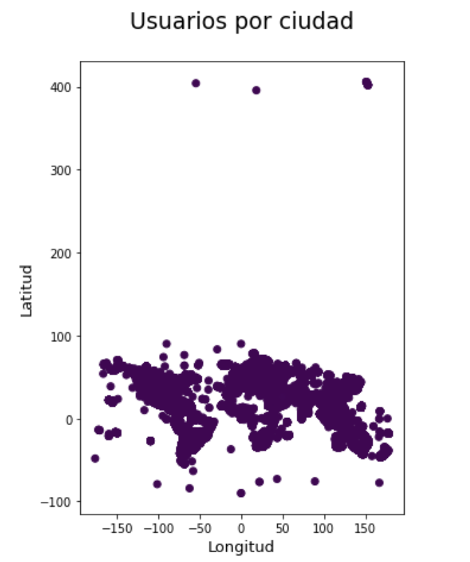
\includegraphics[width=8cm]{dispersion ubivaiones.png}
\centering
\caption{Gráfico Geométrico de los viajes de los usuarios}
\end{figure}


\section{Metodología}

En la figura 2, se muestra una vista general de la metodología utilizada en este trabajo. Esta métodología, se encuentra bastante simplificada en comparación a lo propuesto en \cite{wang2021poi}, esto debido a que las descripciones del método se encontraban inconclusas, por lo que se tomó la idea general para implementar. Esta se detalla a continuación.
\begin{figure}[H]
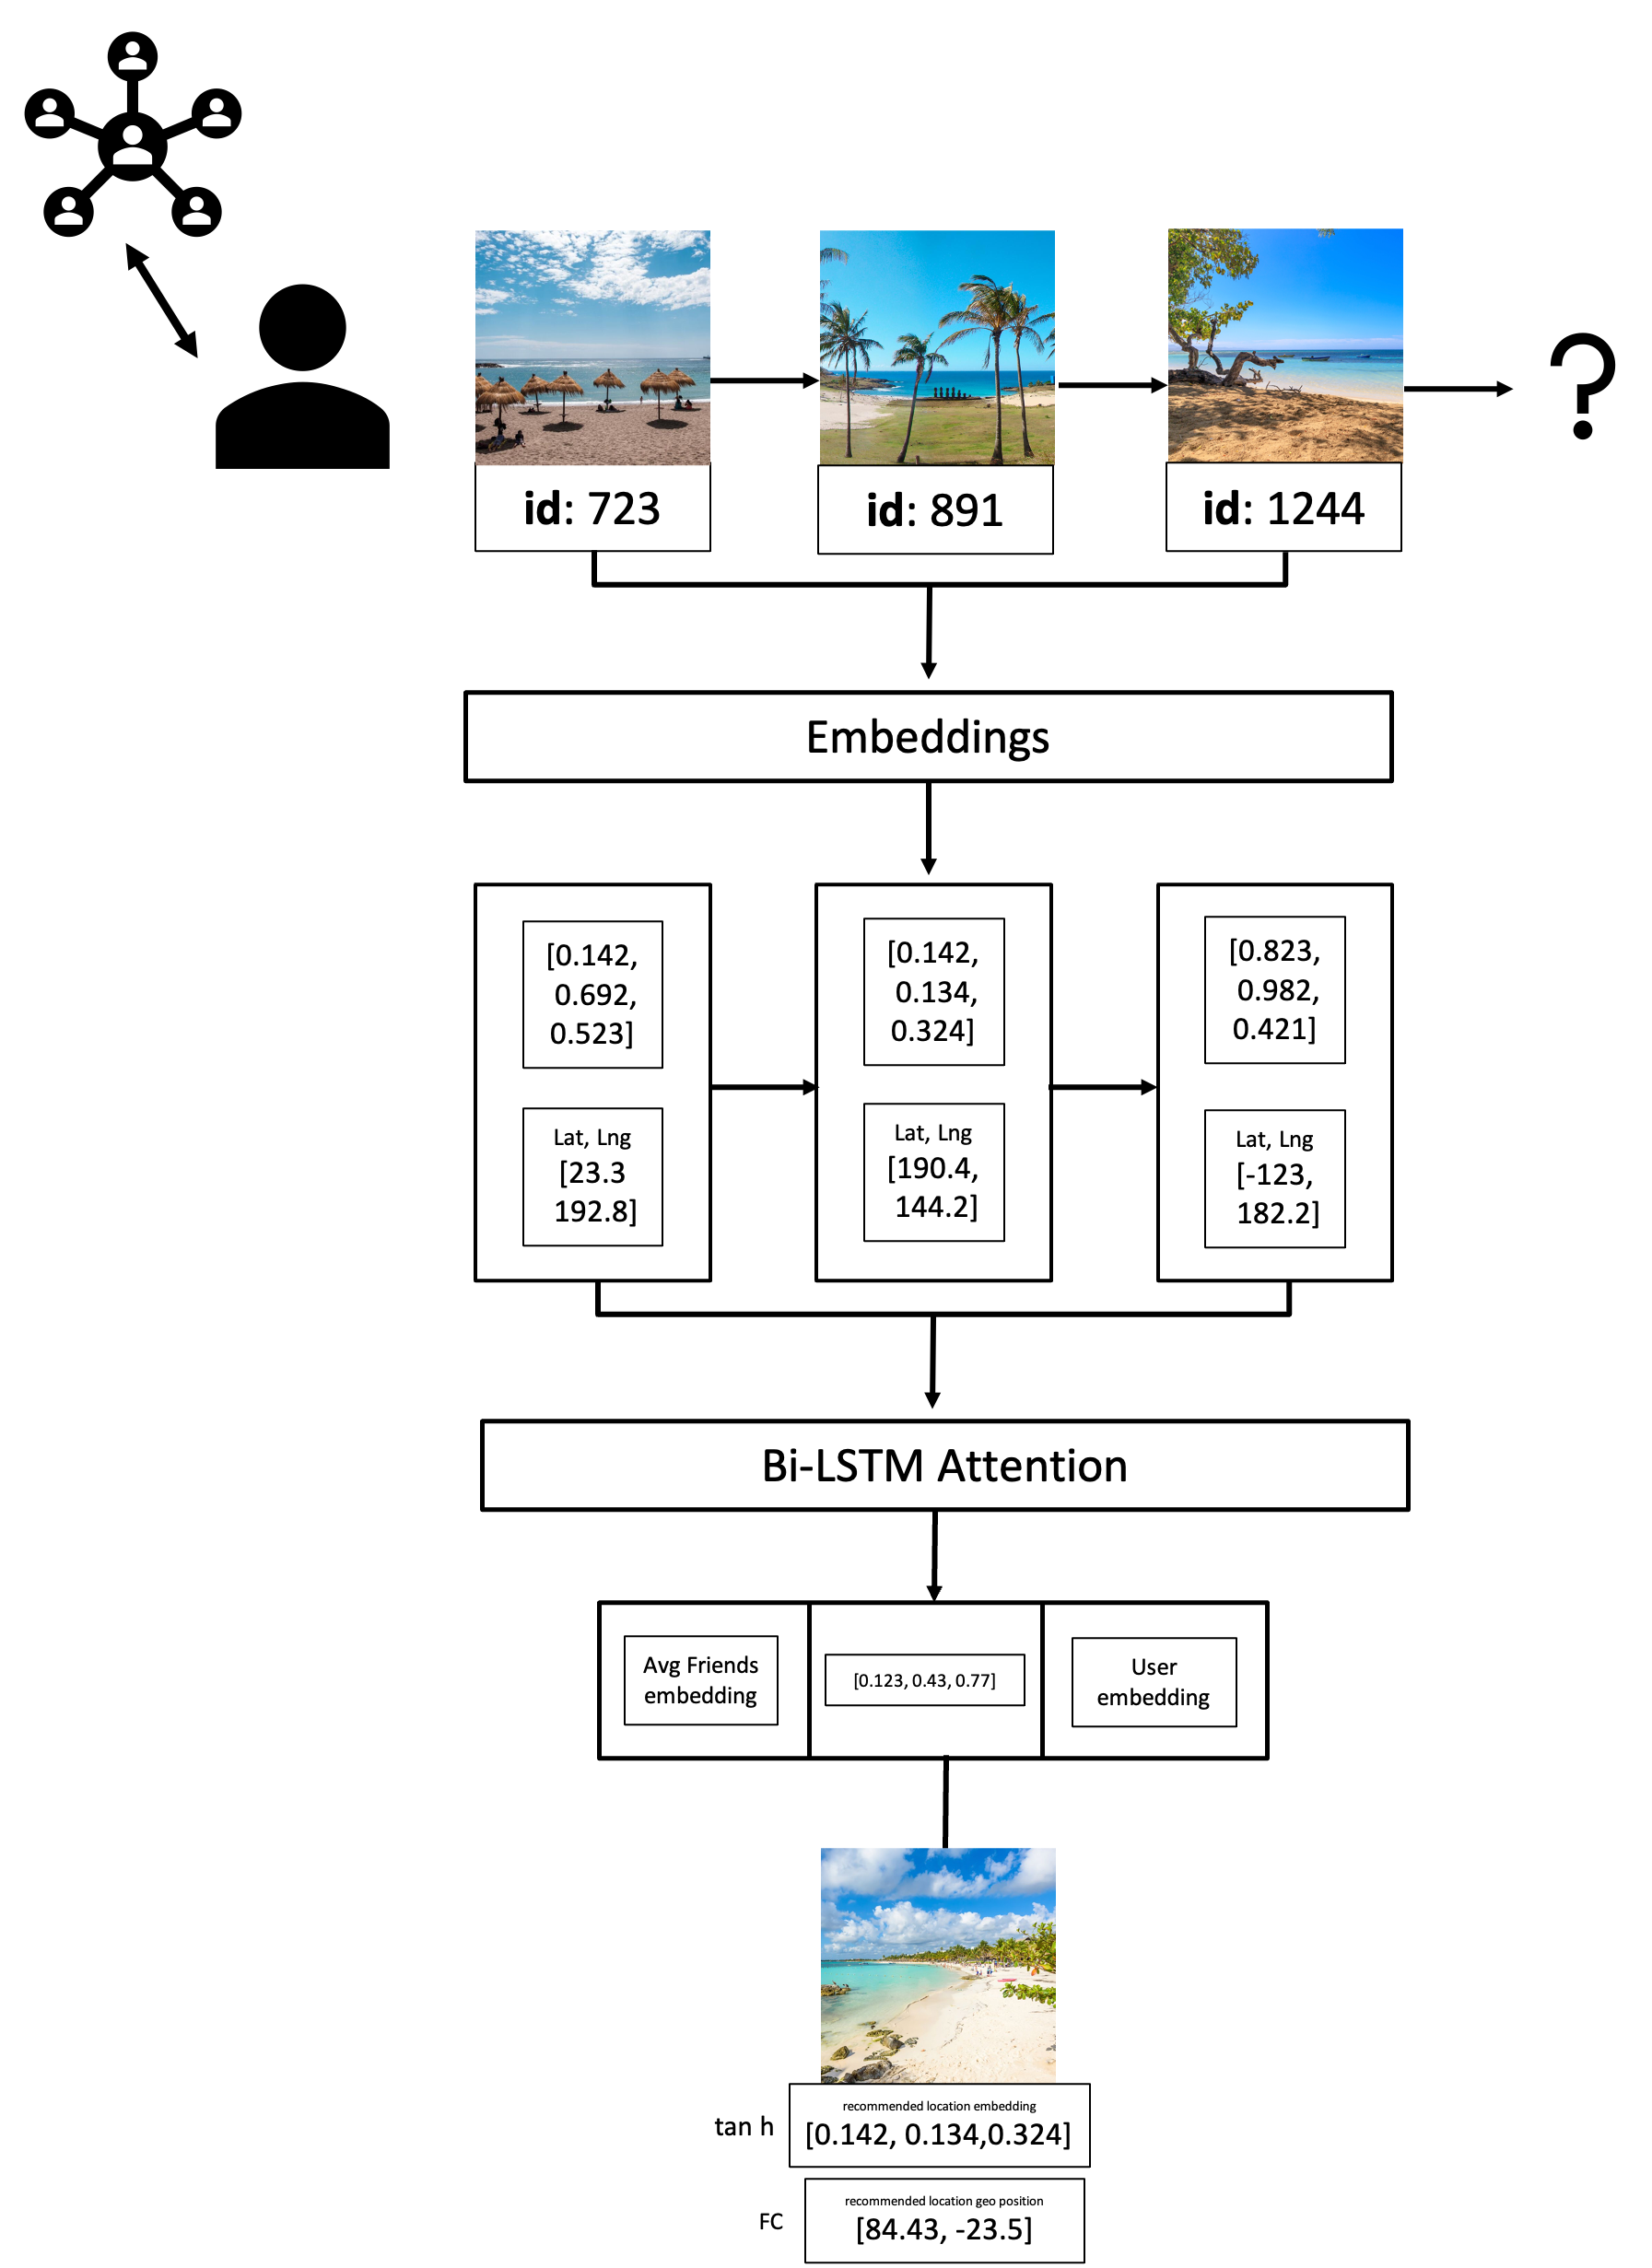
\includegraphics[width=8cm]{diagrama.png}
\centering
\caption{Diagrama métodología modificada}
\end{figure}

\subsection{Embedding Model}
El algoritmo de Word embedding fue propuesto por Bengio et al. en 2003 \cite{bengio2000neural}. Es un modelo de lenguaje natural de una red neuronal de tres capas. El proceso principal es transformar la matriz dispersa en una matriz densa a través de una serie de transformaciones lineales. El propósito es asociar vectores de ubicación independientes, para aprender y obtener automáticamente las conexiones internas entre ubicaciones. En palabras simples, este modelo transforma el id de posiciones en vectores, esta transformación se obtiene entrenando un modelo de lenguaje \cite{bengio2000neural} sobre secuencias de visitas. Así, se logra mapear un espacio semántico que codifica relaciones entre las ubicaciones. 

\subsection{User Embedding}
En el paper base no aparece en detalle que es lo considera al momento de obtener el embedding del usuario, por lo que en este trabajo y para simplificación de la implementación se consideró, el promedio de todas las ubicaciones por las que el usuario ha estado. Este embedding codifica gustos, más no así, secuencias de lugares. 

\subsection{Friends Embedding}
En el mismo caso que user embedding, se considera friends embedding como el promedio de los user embeddings de los amigos del usuario. 

\subsection{Bi-LSTM}

Las redes neuronales recurrentes bidireccionales (RNN) en realidad solo están juntando dos RNN independientes. Esta estructura permite que las redes tengan información hacia adelante y hacia atrás sobre la secuencia en cada paso de tiempo.
\begin{figure}[H]
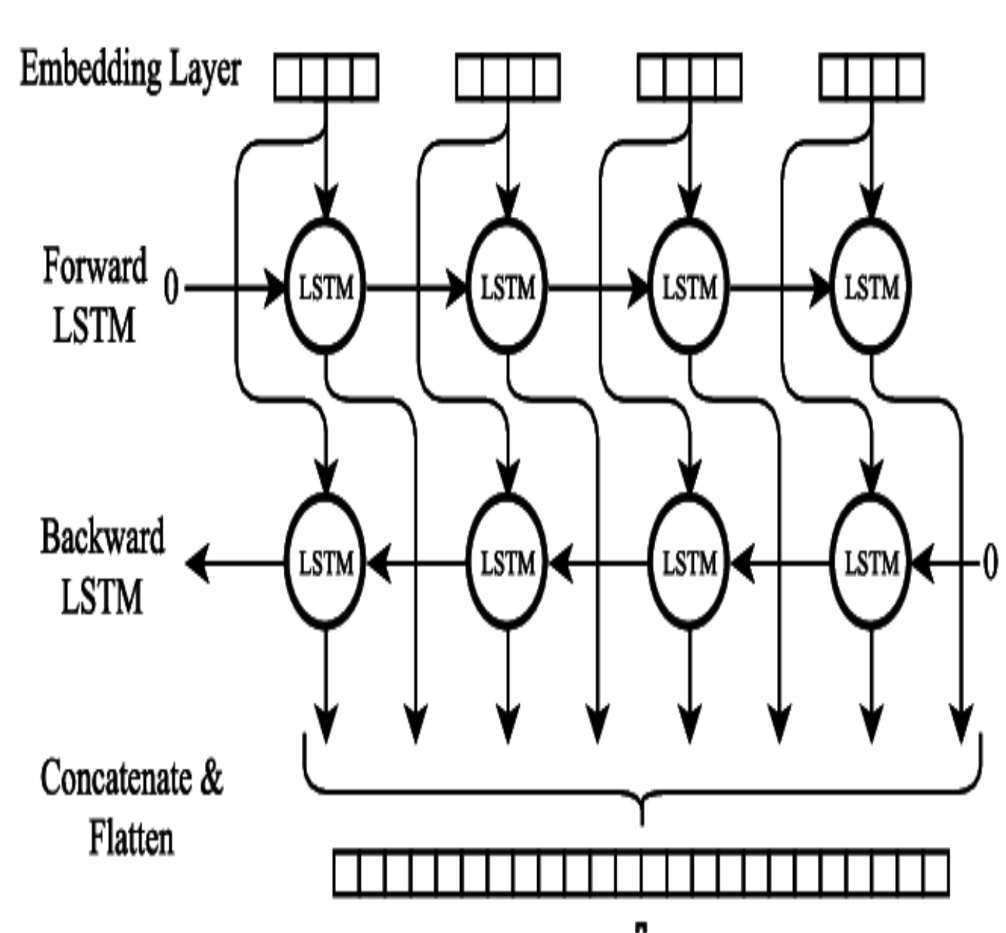
\includegraphics[width=8cm]{Imagen 1.png}
\centering
\caption{Diagrama Bi-LSTM}
\end{figure}
El uso bidireccional ejecutará sus entradas de dos maneras, una del pasado al futuro y otra del futuro al pasado y lo que diferencia este enfoque del unidireccional es que en el LSTM que se ejecuta hacia atrás se conserva la información del futuro y al usar los dos estados ocultos se combina son capaces en cualquier momento de preservar información tanto del pasado como del futuro. \cite{gao2018exploiting}
\subsection{Attention Layer}
El mecanismo de atención es un mecanismo de procesamiento de señales cerebrales similar a la visión humana. Al calcular los pesos de los vectores de características que salen de la red bidireccional de memoria a corto plazo (Bi-LSTM) en diferentes momentos, destacando algunas características importantes, todo el modelo de red puede mostrar un mejor rendimiento. En el reconocimiento de comportamiento, la red neuronal se enfoca en algunas acciones y objetos clave al agregar un mecanismo de atención al entrenar el modelo. Cuando el modelo encuentre este tipo de acciones u objetos la próxima vez, dará prioridad a la predicción de estos comportamientos y reducirá el alcance del reconocimiento. Luego ajuste la distribución del peso de acuerdo con la relación entre las acciones para lograr un reconocimiento más preciso.

\begin{figure}[H]
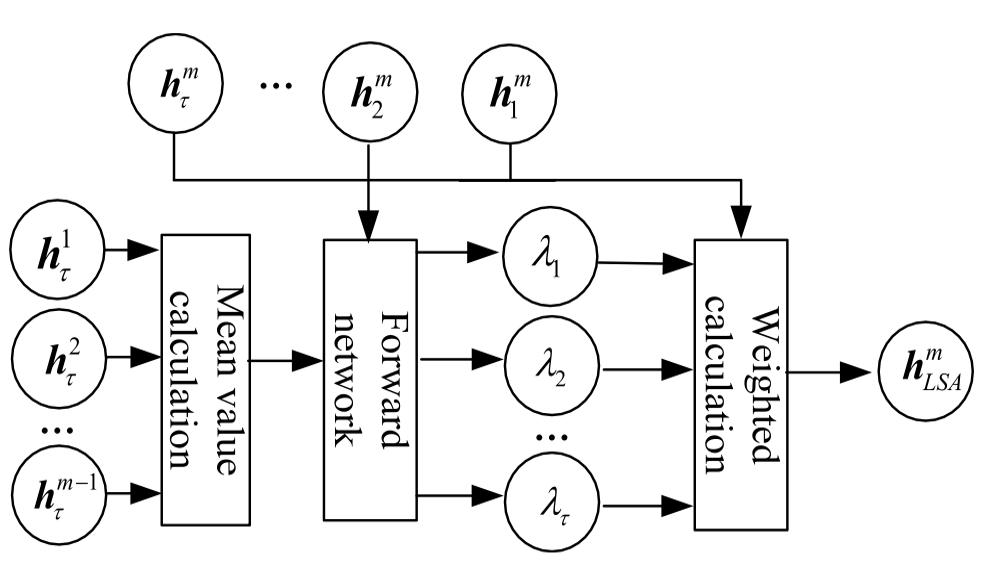
\includegraphics[width=8cm]{attention.png}
\centering
\caption{Diagrama Attention Layer}
\end{figure}
El mecanismo de atención que se muetra en la figura 4, filtra la información clave que es más importante para el objetivo de la tarea actual de un gran cantidad de información. En donde , $\lambda_i$ representa a los pesos del momento del incio del POI.
Para mayor detalle del funcionamiento de esta capa consultar en \cite{wang2021poi}

\subsection{Loss Function}
La función de pérdida del modelo se divide en dos partes: la distancia entre el vector de puntos de interés pronosticado y el vector real y la distancia entre la ubicación geográfica predicha y la ubicación geográfica real. La brecha entre el vector predicho y el vector real puede describir la precisión del vector predicho y es la parte más importante de la función de pérdida. La diferencia entre la ubicación geográfica predicha y la ubicación real también se agrega a la función de pérdida como parte del ajuste. Esto se debe a que la gama de actividades del usuario es limitada y el POI predicho no debe desviarse demasiado de la gama de actividades habitual del usuario. De lo contrario, la recomendación perderá sentido. La función de pérdida específica es la siguiente:
\begin{itemize}
    \item La diferencia entre el vector predicho y el vector real se mide por la similitud del coseno. Dada por la siguiente ecuación: 
    \begin{figure}[H]
    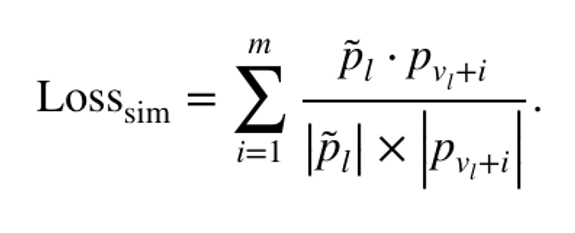
\includegraphics[width=8cm]{losim.png}
    \centering
    \caption{Función de perdida similitud coseno}
    \end{figure}

    \item La distancia euclidiana se utiliza para la similitud entre las ubicaciones geográficas y la ubicación geográfica predicha.
    \begin{figure}[H]
    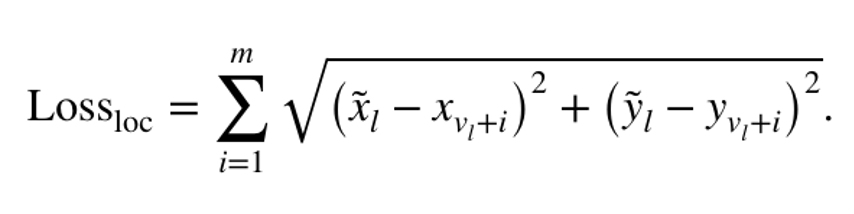
\includegraphics[width=8cm]{losloc.png}
    \centering
    \caption{Función de perdida distancia euclideana}
    \end{figure}
\end{itemize}

Finalmente la función de perdida es la suma de estas dos funciones anteriormente mostradas. 
    
\section{Resultados obtenidos}

\subsection{Método de entrenamiento}

Los modelos expuestos a continuacion fueron entrenados con el optimizador \textit{Adam}, con un \textit{Learning Rate} base de 0,01. Además, para disminuir el \textit{Learning Rate}
se utilizó un \textit{scheduler} que en reduce el \textit{lr} por un factor de 10 cuando han pasado 5 épocas sin que se note un decenso en la mejor \textit{validation loss} vista hasta el momento. También se implementó \textit{Early Stopping}, para detener el entrenamiento en caso de que la \textit{val loss} no mejore por 15 épocas seguidas. \\

Los resultados de todos las ejecuciones de entrenamientos se pueden ver en \cite{wandb}.

\subsection{Modelo de Embeddings}

Se implementó el modelo de embeddings según el paper \cite{bengio2000neural}. Para encontrar la mejor combinación de hiperparámetros, se entrenó el modelo con múltiples combinaciones y luego se comparó según la pérdida del set de validación. Se puede ver en la Tabla 1 que la combinación de \textit{embedding dim} = 16 y \textit{Hidden dim} = 10 otorga la mejor pérdida de validación.  Sin embargo, este no varía demasiado a menos que la dimensión de la capa oculta aumente sustancialmente.  Una expliación a esto puede ser que a mayor número de parámetros es más probable que se produzca \textit{overfitting}. \\

En consecuencia, se entrenó el modelo de embeddings con dichos parámetros y se utilizó para implmentar el resto del modelo. Es bueno recordar que el modelo de embeddings no cambiará sus parámetros al entrenar el modelo propuesto. 

\begin{table}[h]
\begin{center}
\begin{tabular}{| c | c | c|}
\hline
Embedding_dim & Hidden_dim & Val_loss \\ \hline
128 & 150 & 37,334 \\
128 & 80 & 29,147 \\
128 & 40 & 21,302 \\
128 & 20 & 17,439 \\
128 & 10 & 16,223 \\
64 & 150 & 20,263 \\
64 & 80 & 16,955\\
64 & 40 & 16,214\\
64 & 20 & 16,151\\
64 & 10 & 16,116\\
32 & 150 & 16,221\\
32 & 80 & 16,174\\
32 & 40 & 16,122\\
32 & 20 & 16,099\\
32 & 10 & 16,076\\
16 & 150 & 16,148\\
16 & 80 & 16,113\\
16 & 40 & 16,090\\
16 & 20 & 16,087\\
16 & 10 & 16,060\\
\hline
\end{tabular}
\caption{Ajuste de hiperparámetros de modelo de embeddings}
\label{tab:fruta}
\end{center}
\end{table}

\section{Evaluación}

Se comparó el rendimiento del modelo con los métodos \textit{Most Popular} y \textit{Random}. Los resultados están expuestos en la Tabla 2. Se obtuvo una precisión bastante baja de 0,000013. Esto logra vencer al método \textit{Random} por un órden de magnitud, pero es varios ordenes de magnitud menor que \textit{Most Popular}. Como se mencionó anteriormente, esto puede deberse a decisiones de diseño subóptimas, de la mano con que el dataset es extremadamente disperso.

\begin{table}[h]
\begin{center}
\begin{tabular}{| c | c | c|}
\hline
Modelo & Precision  \\ \hline
Most Popular & 0,0043  \\
Random & 0,0000026 \\
Propuesto & 0,000013 \\

\hline
\end{tabular}
\caption{Comparación de rendimiento}
\label{tab:fruta}
\end{center}
\end{table}
\section{Conclusiones}
Se logra implementar un modelo en base al paper propuesto, sin embargo, se tuvieron que tomar decisiones de diseño, que no se encontraban en el paper. Las principales decisiones de diseño fueron las mencionadas en la seccion 4 de metodología, principalmente la opción de embeddings de usuario. 

Todo el código fuente de este paper, tanto implemenatación como este mismo paper, pueden encontrarse en \cite{source}.


\bibliographystyle{ACM-Reference-Format}
\bibliography{sample-base}

\end{document}
\endinput
%%
%% End of file `sample-sigplan.tex'.
